% lab02

\section{Lab 2}
\

!! add something about unimodal/multimodal !!

All the following analysis are done by inspecting visually the
histograms and scatterplots of the data, therefore they aren't quantitative and misurable
evaluations, but just qualitative findings evaluated by eye.
From the figure \ref{fig:scatter} we can extract some valuable informations about the features of our
data.

About the first two features, they are first of all unimodal: this can be useful if we use some
model that assume a distribution that is inherintly unimodal (??even other stuff about data generation
process??).
Additionally, they show a significant overlapping degree: the means per class are very similar, but variances are different.
We can conclude that these two features are less informative than features with much different means,
but, since the different variances, they could still be useful combined with some other feature,
using techniques such as PCA and LDA. In this specific case, since we are taking
into account the discriminatory power of the features, LDA (or a mix of the two techniques)
could be more suitable, but it's not a predictible behaviour. (??)

Moving on the last two, they're are less overlapped compared to the previous ones, but multimodal: multimodality can be challenging,
specifically if we use some parametric model that assume an underlying unimodal distribution, such
as Gaussian Models. So an extrimely simple model in the specific case of these two features could perform poorly.

The third and the fourth features instead are unimodal and have a lower overlapping degree,
so probably, if we use a simple model, they could be the most useful ones. 
Applying LDA moreover, we can notice that the found directions highly correspond
to the directions of the third and the fourth features, since LDA
tend to select linear combination of the features in a way that the first component
is the more "discriminant" for each class.

\begin{center}
    \begin{lstlisting}
        D, L, label_dict = load("project/data/trainData.txt")
        W_lda_m1, D_lda_m1 = lda(D, L, m=1)
        print(W_lda_m1)
        
        # Output:
        #[[-0.01063821]
        # [ 0.0134172 ]
        # [-0.96566604]
        # [ 0.96774246]
        # [ 0.0217633 ]
        # [-0.03289391]]
        
    \end{lstlisting}
\end{center}
    
\begin{figure}[htbp]
    \centering
    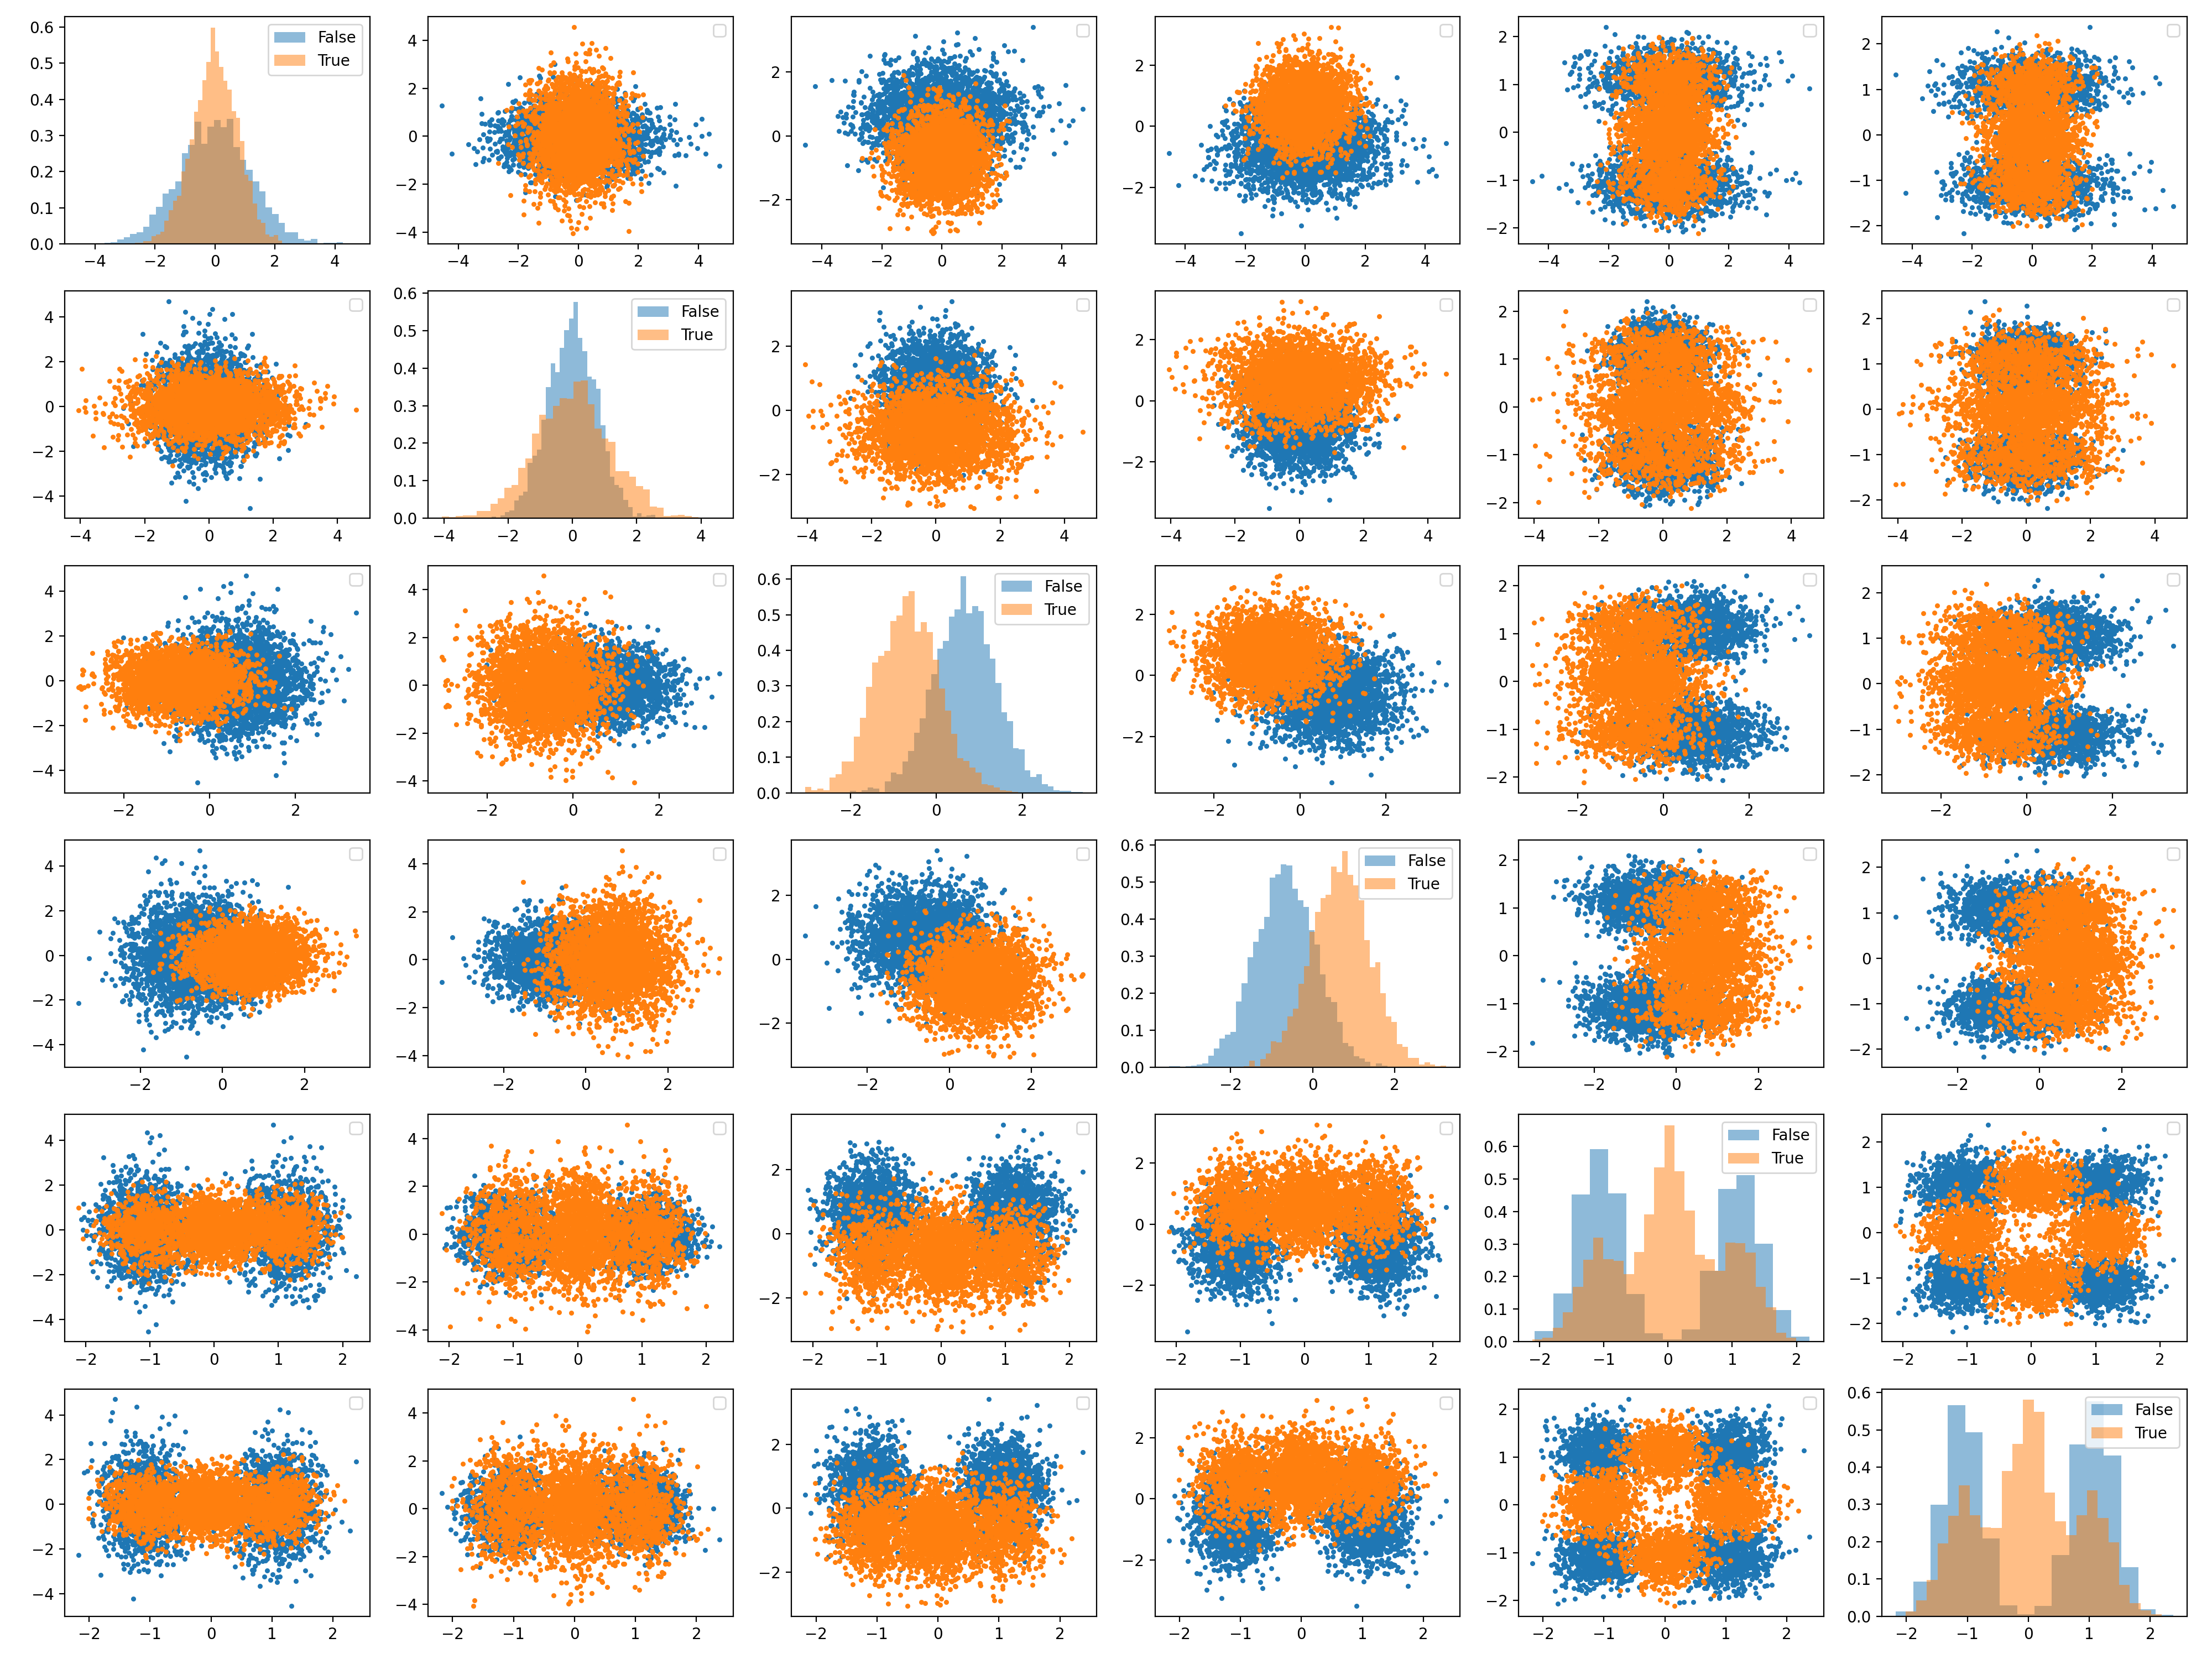
\includegraphics[width=0.9\linewidth]{lab02/scatter.png} % Adjust the width as needed
    \caption{Spoofing dataset scatter and histogram plots}
    \label{fig:scatter}
\end{figure}